\chapter{Теоретическое описание} \label{Theor}
\section{Теоретический подход и феноменология неупорядоченных сверхпроводников}
При микроскопическом описании сверхпроводящего состояния традиционным подходом является БКШ-подобные гамильтонианы на основе точных состояний невзаимодействующей системы электронов:
\begin{equation}
\label{eq:BCS_type_Ham}
H_{BCS} = \sum_{j\sigma} \xi_j a_{j\sigma}^\dagger a_{j\sigma} - \frac{\lambda}{\nu_0} \sum_{ijkl} V_{ijkl} a_{i\uparrow}^\dagger a_{j\downarrow}^\dagger a_{k\downarrow} a_{l\uparrow}
\end{equation}
где использованы следующие обозначения:
\begin{itemize}
	\item $i$ --- индекс одночастичного собственного состояния невзаимодействующей системы c энергией $\xi_j$,
	\item $a_{j\sigma}^\dagger, a_{j\sigma}$ --- фермионные операторы рождения уничтожения соответствующего состояния,  $\sigma$ --- спиновый индекс,
	\item $\nu_0$ --- плотность одночастичных состояний системы,
	\item константа $\lambda$ характеризует притягивающее Куперовское взаимодействие, обрезаемое на некотором энергетическом масштабе $\varepsilon_0$; предполагается, что  зависимостью притягивающего взаимодействия от импульса можно пренебречь, т. е. считать его точечным;
	\item $V_{ijkl}$ содержит в себе информацию о перекрытии уровней и амплитуде туннелирования между этими состояниями
\end{itemize}

Для возможности теоретического рассмотрения задачи необходимо сделать дальнейшие упрощения, касающиеся деталей устройства одночастичных состояний и их перекрытий. К сожалению, до сих пор не построено последовательной теории, позволяющей эти упрощения обосновать и выяснить критерии их применимости, поэтому изложенные ниже предположения в значительной степени будут обоснованы исключительно качественно за счёт феноменологии и экспериментальных данных. Подробное обсуждение модели \eqref{eq:BCS_type_Ham} и постулируемых далее приближений можно также найти в \cite{Feigelman2010}.


\subsection{Преформирование электронных пар}
%ЗДЕСЬ ЕЩЕ ВПИСАТЬ ССЫЛКУ НА SACEPE, FEIGELMAN 2011 NATURE, есть в [7]
%Решил не включать, потому что ссылка на эту работу есть в \cite{Dubouchet_et_al_2018}, и изложено там +- тоже самое. Плюс, МВ кидал ссылку и на \cite{Dubouchet_et_al_2018}, так что все ок.
Для упрощения модели требуется уточнить структуру самих матричных элементов $V_{ijkl}$, для чего мы привлечём экспериментально наблюдаемое явление наличия т. н. псевдощели. Суть данной концепции заключается в видимом присутствии парных электронных образований даже при отсутствии коллективных сверхпроводящих эффектов. Это явление экспериментально обнаруживается по различию спектров одночастичных и двухчастичных возбуждений, выявленных методами туннельной андреевской спектроскопии \cite{Dubouchet_et_al_2018}, а также по данным измерения проводимости в некоторых изоляторах вблизи сверхпроводящего перехода, демонстрирующих термоактивационное поведение сопротивления \cite{Shahar_Ovadyahu_1992}. Важные для рассматриваемой нами модели феноменологические аспекты и выводы из экспериментальных данных для этого явления таковы:
\begin{itemize}
	\item В широком диапазоне температур, включающем в себя температуру сверхпроводящего перехода $T_c$, электроны в системе представлены связанными парами с суммарным нулевым спином, причём каждая пара занимает некоторое одночастичное состояние.
	\begin{itemize}
		\item Причина притяжения, обуславливающего такое поведение, является предметом обсуждения. Хорошим кандидатом выглядит непосредственно само Куперовское притяжение, поскольку локализационный объём одного состояния достаточно большой для развития этого эффекта. Это контролируется параметром $\nu_0 V_{loc} \varepsilon_0 \gg 1$, где $\varepsilon_0$ -- энергетическая обрезка Куперовского притяжения в гамильтониане \eqref{eq:BCS_type_Ham}.
	\end{itemize}
	
	\item Энергия разрыва этих пар $\Delta_P$ значительно превышает все сверхпроводящие масштабы энергий, вроде амплитуды параметра порядка $\Delta$ и температур перехода $T_c$. 
	\begin{itemize}
		\item По существу это означает, что электроны по системе перемещаются в основном парами, что также означает ярко выраженные эффекты чётности. Поскольку нашей исходной задачей является описание низкоэнергетической физики системы, то логичным предположением будет исключение одночастичных состояний из рассмотрения, и учёт лишь динамики состояний электронных пар.
	\end{itemize}
\end{itemize} 
Исходя из этих фактов, нашу модель можно дополнить следующими приближениями, упрощающими структуру члена со взаимодействием в гамильтониане \eqref{eq:BCS_type_Ham}.
\begin{itemize}
	\item В динамике системы участвуют только состояния с числами заполнения $n_i = 0\text{ или }2$, поскольку состояние с $n_i = 1$ отделено большой щелью.
	\item Соответственно, мы можем допустить, что основную роль играют процессы прыжков электронных пар между состояниями, так что из всех матричных элементов в гамильтониане \eqref{eq:BCS_type_Ham} мы оставим только полудиагональные вида $V_{iijj}$.
	\item Диагональные матричные элементы $V_{iiii}$, описывающие самовзаимодействие, мы также считаем нулевыми (считаем, что их эффект сводится к перенормировке энергии узла). 
\end{itemize}


\subsection{Одночастичная локализация точных состояний}
Поскольку образцы, в которых наблюдается исследуемый нами феномен наличия низкоэнергетических возбуждений, при температурах выше температуры перехода демонстрируют свойства изолятора, то это свидетельствует о проявлении в этих образцах эффектов одночастичной локализации Андерсона. Феноменология этого эффекта уже хорошо изучена, обзор основных результатов можно найти, например, в \cite{Lee_Ramakrishnan_1985}. Качественно важные для нас свойства Андерсоновской локализации можно резюмировать следующим образом: 
\begin{itemize}
	\item при достижении силы беспорядка (например, концентрации примесей) некоторого критического значения одночастичные волновые функции электронов перестают быть делокализованными по всему образцу (как это было бы в случае Блоховских волновых функций), и обретают некоторый конечный локализационный объём, за пределами которого их амплитуда экспоненциально мала.
	\item В широком диапазоне значения силы беспорядка (в т. ч. ниже критического) волновые функции характеризуются так называемой фрактальной структурой, которая количественно описывается степенной зависимостью от занимаемого объёма различных моментов амплитуды волновой функции с нетривиальным показателем:
	$$
	P^{(q)} := \left\langle |\psi_i(r)|^q \right\rangle \sim V_{loc}^{d_q}
	$$
	где усреднение ведётся по координате $r$, пробегающей весь объём образца. Качественно это поведение означает, что волновая функция сложным (самопободобным) образом хорошо выражена лишь в части занимаемого ей объёма.
	\item Перекрытия состояний также приобретают фрактальную статистику, характеризуемую степенной зависимостью перекрытий от разности энергий $\xi_i$ соответствующих состояний:
	$$
	C_{ij} := \left\langle \psi_i(r) \psi_j^{*}(r) \right\rangle \sim \left| \xi_i - \xi_j \right|^{d_{overlap}}
	$$
\end{itemize}
Подробное обсуждение этих эффектов также имеется в \cite{Feigelman2010}. К сожалению, строгий учёт этих эффектов представляется весьма трудоёмкой процедурой, не позволяющей до сих пор выделить ключевые феноменологические аспекты. Поэтому предлагается сделать качественные упрощения, которые сохраняют предположительно существенную феноменологию:
\begin{itemize}
	\item будем считать, что система находится неглубоко в фазе изолятора, т. е. в таких условиях, когда локализационный объём $V_{loc}$ уже не является макроскопической величиной порядка размеров  реальных систем, однако он все ещё содержит в себе большое количество одночастичных состояний, позволяя развиваться механизмам Куперовского притяжения, что контролируется параметром $\nu V_{loc} \epsilon_0 \gg 1$.
	\item Абсолютная величина перекрытия состояний воспроизводится довольно грубо: в рамках нашей модели перекрытие или имеется с некоторой постоянной амплитудой, не зависящей от выбранной пары узлов, или не имеется вовсе. Мы заменяем, вообще говоря, нетривиальное и коррелированное между различными парами узлов распределение совокупности матричных элементов $V_{iijj}$ в гамильтониане \eqref{eq:BCS_type_Ham} на его сильно упрощённый вариант, делящий все пары состояний на связанные и несвязанные. При этом характерным значением, определяющее это разделение, естественным образом будет являться энергия Куперовского притяжения.
	\item Учёт фрактальной структуры волновых функции внутри локализационного объёма мы также проведём очень качественно: будем считать, что у каждого узла имеется некоторое большое \textit{постоянное} число $K + 1 \gg 1$ ненулевых перекрытий \textit{случайно выбранным множеством состояний}. Разумеется, последнее предположение нарушает локальные свойства модели, потенциально разрешая перекрытия между двумя очень далёкими в реальном пространстве состояниями, однако здесь мы предполагаем, что ни флуктуации реального числа перекрытий от узла к узлу, ни  прыжки на большие расстояния не определяют реальную физику происходящего процесса.
	\item Плотность состояний невзаимодействующей системы мы будем моделировать простым распределением ширины $W \sim E_F$ с ненулевой плотностью состояний в центре зоны. Данное приближение обосновано постольку, поскольку по сравнению с характерным масштабом изменения плотности состояний (этот масштаб как раз $\sim E_F$) все прочие энергетические величины, не превышающие обменной энергии Куперовского взаимодействия $\varepsilon_0 \ll E_F$ пренебрежимо малы, так что изменением плотности состояний можно не учитывать. 
\end{itemize}
Подчеркнём, что приближения, моделирующие статистику перекрытий состояний, являются очень качественными, так как любые уточнение в сторону более точной картины на данный момент не позволяют добиться построения решаемой модели. Мы надеемся, что основная физика явления доставляется лишь тем фактом, что каждый узел связан с большим числом прочих узлов с близкими между собой значениями туннельных амплитуд, каждая из которых порядка энергии Куперовского взаимодействия $\varepsilon_0$, а редко встречающиеся флуктуации (их редкость, вообще говоря, тоже весьма условна) не являются определяющими.


\subsection{Итоговая модель}
Перед окончательной формулировкой модели дадим ещё один небольшой комментарий: гамильтониан \eqref{eq:BCS_type_Ham} не учитывает Кулоновское взаимодействие электронов. Количественная степень обоснованности этого пренебрежения до сих пор понята очень плохо, и основные аргументы в пользу такого приближения апеллируют к экспериментальным фактам, основным из которых является независимость поведения псевдощели и истинного параметра порядка при сверхпроводящем переходе, в то время как Кулоновское взаимодействие должно подавлять оба явления одинаковым образом. С имеющимися точками зрения а также основными аргументами в пользу пренебрежения Кулоновским взаимодействия можно ознакомиться в \cite{Feigelman2010}.

Резюмируя все рассуждения выше, можем перечислить итоговые предположения рассматриваемой в этой работе модели:
\begin{enumerate}
	\item Электроны во всём существенном для задачи диапазоне температур образуют пары с нулевым суммарным спином, каждая из которых занимает некоторое одночастичное состояние и физически локализована в конечном объёме.
	\item Разрывом этих пар в задаче можно пренебречь.
	\item Кулоновское взаимодействие также можно не учитывать.
	\item Перемещения электронов описываются прыжками пар между состояниями.
	\item Каждое состояние имеет \textit{постоянное} перекрытие с большим \textit{постоянным} числом соседей $Z = K + 1 \gg 1$.
	\item Соседствующие между собой узлы выбираются \textit{случайным} образом, без какой-либо регулярной структуры.
	\item Энергии парных состояний можно считать некоррелированными случайными величинами, подчиняющимися некоторому распределению конечной большой ширины $W \sim E_F$.
	\item В дальнейшем мы будем интересоваться низкотемпературным поведением модели
\end{enumerate}
Данные утверждения позволяют записать практически окончательную форму гамильтониана:
\begin{equation}
\label{eq:Ham_physical}
H_{model} = \sum_{j\sigma} \xi_j a_{j\sigma}^\dagger a_{j\sigma} - \frac{g}{K} \sum_{(ij)} a_{i\uparrow}^\dagger a_{i\downarrow}^\dagger a_{j\downarrow} a_{j\uparrow}
\end{equation}
где
\begin{itemize}
	\item $i,j$ --- узлы некоторого случайного $K$-регулярного графа (т. е. такого графа, у которого число соседей каждой вершины постоянно и равно $Z = K + 1$) с термодинамическим большим числом узлов $M$, а сумма в члене со взаимодействием происходит по рёбрам этого графа;
	\item $\xi_i$ --- энергии соответствующих состояний, представляемые \textit{независимыми одинаково распределенными случайными величинами} с плотностью распределения $P(\xi) = \frac{1}{2 W}\theta(W - |\xi|)$; заметим, что величина $W$ также определяет плотность состояний в невзаимодействующей системе: $\nu_0 \cdot 2 W = 1$;
	\item Сила взаимодействия определяется константой $g$, вбирающей в себя характеристики силы Куперовского спаривания и перекрытия состояний. Лишний множитель $1/K$ во взаимодействии призван корректно воспроизводить предел чистого сверхпроводника (по существу, он также является частью величины перекрытия состояний).
\end{itemize} 

Далее являются удобными следующие упрощения:
\begin{itemize}
	\item переход на новые энергетические единицы $W$, что избавляет от лишней константы, и потому можно положить
	$$
	P(\xi) = \frac{1}{2}\theta(1 - |\xi|)
	$$
	\item введение так называемых псевдоспиновых операторов, осуществляющих отображение на задачу системы взаимодействующих спинов $s = 1/2$ на случайном графе:
	\begin{align}
	\label{pseudospin_op}
		2s^z_j & = \sum_\sigma a_{j\sigma}^\dagger a_{j\sigma} - 1 &
		s^+_j & = a_{j\downarrow}^\dagger a_{j\uparrow}^\dagger &
		s^-_j & = a_{j\downarrow} a_{j\uparrow}
	\end{align}
\end{itemize}
В результате этих упрощений, окончательное выражение имеет хорошо известный вид т. н. псевдоспинового гамильтониана \cite{Ma_Lee_1985}:
\begin{equation}
\label{eq:Ham_final}
H_{PS} = \sum_{j} 2 \xi_j s_j^z - \frac{g}{K} \sum_{(ij)} (s_i^+ s_j^- + h.c) \equiv \sum_{j} 2 \xi_j s_j^z - \frac{2g}{K} \sum_{(ij)} (s_i^x s_j^x + s_i^y s_j^y)
\end{equation}
Таким образом, поставлена задача об изучении устройства основного состояний и элементарных возбуждений гамильтониана \eqref{eq:Ham_final}.

В заключение сделаем важное физическое замечание: гамильтониан \eqref{eq:Ham_final} \textit{полностью исключает из задачи} детали устройства одночастичных состояний в реальном пространстве. Поэтому полученные в рамках этой модели ответы, должны интерпретироваться, строго говоря, только в сочетании со знанием статистики взаимного расположения одночастичных состояний в реальном пространстве.



\section{Основные уравнения теории сверхпроводимости}
\subsection{Представление семионов Попова-Федотова}
Отправной точкой построения функционального интеграла для псевдоспинового гамильтониана \eqref{eq:Ham_final} будет являться хорошо известное \textit{семионное представление Попова-Федотова} \cite{Popov_Fedotov}. 
%Более полный формализм, обобщающий данное представление, а также дающий полезные математические сведения касательно этого метода, можно найти в \autoref{App_Semion}. 
Эта техника получила обобщение на случай произвольного спина $s$ (с некоторыми оговорками), с примером её применения в общем виде можно ознакомиться, например, в \cite{Veits_etal_1994}. В этой работе же будут даны только необходимые для дальнейшего вывода сведения.

\subsubsection{Определения}
Рассмотрим стандартное представление спиновой алгебры $\mathfrak{su}_2$ со спином $s = 1/2$.
\begin{itemize}
	\item Спиновые операторы будем обозначать маленькими буквами: $s^x, s^y, s^z$. Эти операторы весьма очевидным образом связаны с матрицами Паули. Элементы алгебры мы будем далее отождествлять с их каноничным представлением.
	\item Пространство состояний, на котором строится представление, обозначим $V^S$. В качестве базиса возьмём собственные вектора оператора $z$-проекции спина: $\left\{ \left|s, m\right>: m\in[-s,s] \right\}$. Полная размерность пространства, очевидно, равна $\dim V^S = 2s+1$.
	\item Коммутационные соотношения в алгебре стандартны: $ \left[ s^i, s^j \right]_{-} = i \epsilon^{ijk} s^k $.
\end{itemize}
Введём также алгебру $\mathfrak{f}$ операторов рождения и уничтожения фермионов, которые могут находиться в одном из $2s+1 = 2$ состояний.
\begin{itemize}
	\item Операторы рождения и уничтожения фермиона в соответствующем состоянии будем нумеровать нижним индексом:	$\left\{ c_k, c_k^\dagger: k\in[-s,s] \right\} $
	\item Полное Фоковское пространство состояний, обозначим как $V^F$. Базисными векторами в этом пространстве будут собственные вектора оператора числа частиц в конкретном состоянии: $\left\{ \left| n_1,...n_{2s+1} \right>: n_k \in \{0, 1\} \right\}$. Полная размерность есть $\dim V^F = 2^{2s+1} = 4$
	\item Фермионные операторы обладают стандартными правилами коммутации с обычными антикоммутационными соотношениями	$\left\{ c_i, c^\dagger_j \right\}_{+} = \delta_{ij} $, 
	где $\{a,b\}_{+} =: ab + ba$ --- антикоммутатор.
	\item Здесь нам также понадобятся инвариантные подпространства оператора полного числа частиц
	$$N = \sum_{k = -s}^{s} c^\dagger_k c_k \equiv \sum_{k = -s}^{s} N_k$$.
	Подпространство с полным число частиц $n$ мы будем обозначать за $V^F_n$, а базисные вектора это подпространства, являющиеся подмножеством полного набора базисных векторов, мы переобозначим так, что будем указывать там множество занятых состояний: 
	$$\left\{ \left| B \right>: B \subset \overline{\{1,n\}}, |B| = n, N_k \left| B \right> = \begin{cases}
	1, & k\in B\\
	0, & k\notin B
	\end{cases}  \right\}$$
	Очевидно, размерность соответствующего подпространства $\dim V^F_n = C_{2s+1}^n$. Конкретно в случае $s = 1/2$ имеем три подпространства $\dim V^F_0 = 1$, $\dim V^F_1 = 2$,  $\dim V^F_2 = 1$.
\end{itemize} 

\subsubsection{Запись представления}
Представление определяется следующим оразом: каждому оператору $a \in \mathfrak{su}_2$ сопоставляется оператор $A \in \mathfrak{f}$ по формуле
\begin{equation}
\label{eq:semion_repr}
A = \sum_{m, n = - s}^s c^\dagger_m \left\langle m \left| a \right| n \right\rangle c_n
\end{equation}
Для этого представления выполнены следующие важные свойства:
\begin{itemize}
	\item на подпространстве $V^F_1$ ферминонного пространства состояний осуществляется мономорфизм представления спиновой алгебры в представление фермионной Иными словами, на $V^F_1$ матричные элементы соответствующих операторов одинаковые:
	$$ \left\langle {m} \left| A \right| {n} \right\rangle =  \left\langle m \left| a \right| n \right\rangle $$
	Это очевидно из построения.
	
	\item Для $s = 1/2$ верно дополнительно следующее: на ортогональном дополнении к физическому пространству состояний $\left( V^F_1 \right)^\perp$ все операторы вида \eqref{eq:semion_repr} тождественно равны нулю:
	$$ A \left| 1, 1\right\rangle = A \left| 0, 0 \right\rangle = 0$$
	Это является следствием того факта, что представление алгебры $\mathfrak{su}_2$ --- бесследовое: $ \Tr s^i = 0 $.
	
	\item Наконец, если теперь рассмотреть тензорное произведение алгебр, соответствующей, скажем, локальным операторам на узлах графа, то очевидным является распространение вышеуказанных утверждений и на этот случай. Иными словами, это представление без изменений применимо и для системы спинов.
\end{itemize}

\subsubsection{Воспроизведение статистических свойств}
Полученное представление даёт возможность взаимно однозначно отобразить задачу исследования равновесной термодинамики псевдоспинового гамильтониана \eqref{eq:Ham_final} на оную для взаимодействующей системы фермионов с тем же парным взаимодействием. Формально это выглядит следующим образом:
\begin{enumerate}
	\item Пусть имеется произвольный спиновый гамильтониан $H^S$, действующий на пространстве состояний некоторого множества спинов $s = 1/2$. Сопоставим ему фермионный гамильтониан $H^F$, получаемый из $H^S$ формальной заменой всех спиновых операторов на фермионные по формуле \eqref{eq:semion_repr} (ну или же можно применить формулу \eqref{eq:semion_repr} сразу ко всему гамильтониану $H^S$, рассматривая при этом тензорное произведение представлений алгебры на узле). Тогда статистические суммы для спинового гамильтониана отличается лишь фазовым множителем от статистической суммы фермионного гамильтониан с мнимым хим. потенциалом $\mu_0 = \frac{i \pi}{2 \beta}$:
	$$
	Z^S(\beta) := \Tr \exp \left\{-\beta H^S\right\} = i^M \Tr \exp \left\{ -\beta H^F + \beta \mu_0 N\right\} =: i^M \mathcal{Z}^F(\beta, \mu_0)
	$$
	где $M$ --- полное число узлов в системе, а $\beta \equiv \frac{1}{T}$ --- обратная температуры. Обратим ещё раз внимание, что в левой части равенства след берётся по спиновому пространству состояний, а в правом --- по полному Фоковскому пространству фермионов.
	\item Немедленным следствием предыдущего утверждения является важное для практического применение утверждение о совпадении средних: среднее \textit{любого} оператора $x$ на системе спинов (будь то одного оператора спина, или любого их произведения) совпадает со средним для оператора $X$, получаемого из $x$ формальной заменой спиновых операторов по формуле \eqref{eq:semion_repr}, с таким же образом полученным фермионным гамильтонианом с мнимым хим. потенциалом:
	\begin{equation}
		\label{eq:semion_mean_correspondence}
		\left\langle x \right\rangle := \frac{\Tr\left[ x \exp\left\{-\beta H^S\right \} \right]}{Z^S} =  \frac{\Tr\left[ X \exp\left\{-\beta H^F + \beta \mu_0 N\right\} \right]}{\mathcal{Z}^F} =: \left\langle X \right\rangle
	\end{equation}
	Это легко увидеть, рассмотрев производящую функцию средних, которая также является стат. суммой некоторого гамильтониана.
\end{enumerate}

\subsubsection{Формулировка исходной задачи в терминах семионов}
Резюмируем полученный результат конкретно для интересующего нас случая: вместо исходной системы \eqref{eq:Ham_final} можно рассматривать равновесную термодинамику следующего фермионного гамильтониана
\begin{equation}
	\label{eq:Ham_semion}
	H_{PS}^F = \underset{H^F_0}{\underbrace{ \sum_{j} \xi_j \sigma^z_{\alpha \beta} c^\dagger_{j\alpha} c_{j\beta} }} \underset{H^F_{int}}{\underbrace{ - \frac{2g}{K} \sum_{(ij)} \frac{1}{4} \left( \sigma^x_{\alpha \beta} \sigma^x_{\rho \eta} + \sigma^y_{\alpha \beta} \sigma^y_{\rho \eta} \right) c^\dagger_{i\alpha} c_{i\beta} c^\dagger_{j\rho} c_{j\eta} }}
\end{equation}

Пояснения:
\begin{itemize}
	\item $c^\dagger_{j\alpha},  c_{j\alpha}$ --- операторы рождения и уничтожения фермиона на узле $j$ в состоянии $\alpha$. Таким образом, подразумевается, что на каждом узле имеется $2s+1 = 2$ внутренних состояния, в которых может находиться фермион. 
	
	\item $\sigma^i_{\alpha\beta}$ --- матрицы Паули, воспроизводящие матричные элементы соответствующих спиновых операторов в каноничном базисе собственных состояний $z$-проекции спина. Во всей записи по повторяющимся греческим индексам подразумевается суммирование. Таким образом, мы получили систему фермионов с \textit{парным локальным взаимодействием}.
	
	\item В формуле также явно отражён факт разделения на голый гамильтониан фермионов $H^F_0$ и член взаимодействия $H^F_{int}$.
	
	\item Более общо, любому оператору исходной задачи с псевдоспиновым гамильтонианом \eqref{eq:Ham_final} ставится в соответствие его семионное представление посредством замены каждого спинового оператора по правилу \eqref{eq:semion_repr}.
	
	\item При этом в статистической сумме хим. потенциал принимает чисто мнимое значение $\mu_0 = \frac{i \pi}{2 \beta}$.
\end{itemize}


\subsection{Функциональный интеграл для псевдоспинового гамильтониана}
Благодаря построенному семионному представлению, к задаче теперь можно применять методы функционального интегрирования. Функциональный интеграл по фермионным переменным для многочастичной задачи строится стандартным образом \cite{Altland_Simons}.
\begin{enumerate}
	\item Введём набор Грассмановых антикоммутирующих переменных, соответствующих операторам рождения и уничтожения исходной задачи
	\begin{equation}
		\label{eq:Grassman_field_def}
		\begin{split}
			& \left\{ \overline{\psi}_{i\alpha}, \psi_{i\alpha}: \alpha \in \overline{[-s,s]}, i \in \overline{1,M}\right\} \\
			& \forall i,j,\alpha,\beta \hookrightarrow
			\left\{  \psi_{i\alpha}, \psi_{j\beta} \right\} _{+} = 
			\left\{  \overline{\psi}_{i\alpha}, \psi_{j\beta}  \right\} _{+} = 
			\left\{  \overline{\psi}_{i\alpha}, \overline{ \psi_{j\beta} } \right\} _{+} = 0
		\end{split}
	\end{equation}
	
	\item Определим функцию Гамильтона от этих переменных, которая получается формальной подстановкой $c^\dagger_{i\alpha} \mapsto \overline{\psi}_{i\alpha}, c_{i\alpha} \mapsto \psi_{i\alpha}$ в \textit{нормально упорядоченный} фермионный гамильтониан \eqref{eq:Ham_semion}. К счастью, благодаря тому, что в рассматриваемой системе узел не взаимодействует непосредственно сам с собой (во взаимодействии нет слагаемых с $i = j$), за счёт нормального упорядочения новых членов не появится, так что упомянутая функция будет иметь вид
	\begin{equation}
		\label{eq:Ham_grassman}
		H^G\left( \overline{\psi}, \psi \right) = \underset{H_0^G}{\underbrace{ \sum_{j} \xi_j \tau^z_{\alpha \beta} \overline{\psi}_{j\alpha} \psi_{j\beta} }} \underset{H_{int}^G}{\underbrace{ - \frac{2g}{K} \sum_{(ij)} \frac{1}{4}(\sigma^x_{\alpha \beta} \sigma^x_{\rho \eta} + \sigma^y_{\alpha \beta} \sigma^y_{\rho \eta}) \overline{\psi}_{i\alpha} \psi_{i\beta} \overline{\psi}_{j\rho} \psi_{j\eta} }}
	\end{equation}
	где снова явно отражено разделение членов, аналогичное \eqref{eq:Ham_semion}.
	Требуется также ввести функцию числа частиц
	\begin{equation}
		\label{eq:N_grassman}
		N^{G}\left( \overline{\psi}, \psi \right) = \sum_{j} \overline{\psi}_{j\alpha} \psi_{j\alpha}
	\end{equation}
	
	\item Для определения функционального интеграла отрезок $[0,\beta]$ мнимого Мацубаровского времени разбивается на $N_0 \rightarrow \infty$ одинаковых кусков, и поля $\overline{\psi}_{i\alpha}, \psi_{i\alpha}$ имеют на участке $\left[ (n-1)\frac{\beta}{N_0}, n\frac{\beta}{N_0} \right]$ значение соответственно $\overline{\psi}_{i\alpha}[n], \psi_{i\alpha}[n]$. Грассмановы поля починяются условию антипериодичности 
	\begin{equation}
		\label{eq:Psi_boundary_cond}
		\psi_{i\alpha}(\tau=0) \equiv \psi_{i\alpha}[n = 0] = - \psi_{i\alpha}[n = N_0] \equiv -\psi_{i\alpha}(\tau=\beta),
	\end{equation}
	и аналогично для сопряжённого поля $\overline{\psi}_{i\alpha}$.
	
	\item Вводится мера функционального интегрирования
	$$
	D\left(\overline{\psi},\psi\right) = \prod_{n = 0}^{N_0 - 1} \prod_{i = 1}^{M} \prod_{\alpha = 1}^{2} d\overline{\psi}_{i\alpha}[n] d\psi_{i\alpha}[n]
	$$
	и действие (вес функционального интегрирования)
	\begin{equation}
		\label{eq:Action_discretized}
		\begin{split}
			\mathcal{A} \left[\overline{\psi}, \psi\right] & = \frac{\beta}{N_0} \sum_{k = 0}^{N_0 - 1}  \left[ \frac{\overline{\psi}_{i\alpha}[n] - \overline{\psi}_{i\alpha}[n + 1]}{\beta/N_0} \psi_{i\alpha}[n] - \right. \\ 
			& \left. -  H^{G}\left(\overline{\psi}[n+1],\psi[n] \right) + \mu_0 N^{G}\left(\overline{\psi}[n+1],\psi[n] \right) \right]
		\end{split}
	\end{equation}
	
	\item Наконец, статистическая сумма посредством использования аппарата когерентных состояний \cite{Altland_Simons} выражается через функциональный интеграл:
	\begin{equation}
		\label{eq:Part_sum_discretized}
		\mathcal{Z}^{F} = \lim_{N_0 \rightarrow \infty} \int \limits_{\mathbb{R}} D\left(\overline{\psi}, \psi\right) \exp\left\{ - \mathcal{A} \left[\overline{\psi}, \psi\right] \right\}
	\end{equation}
	Это выражение также принято записывать в виде непрерывного перехода:
	\begin{align}
		\label{eq:Part_sum_func_int}
		\mathcal{Z}^{F} & = \int \limits_{ \begin{array}{cc}
			\psi(0) = - \psi(\beta)\\
			\overline{\psi}(0) = - \overline{\psi}(\beta)
			\end{array} } 
		D\left(\overline{\psi},\psi\right) \exp\left\{ -\mathcal{A} \left[\overline{\psi}, \psi\right] \right\} \\
		\label{eq:Action}
		\mathcal{A} \left[\overline{\psi}, \psi\right] & = \int\limits_{0}^{\beta} d\tau \left[\sum_{i} \frac{\partial \overline{\psi}_{i\alpha} }{ \partial \tau } \psi_{i\alpha} - H^{G}\left(\overline{\psi},\psi\right) + \mu_0 N^{G}\left(\overline{\psi},\psi\right) \right]
	\end{align}
	В такой записи надо иметь в виду, что поля $\overline{ \psi}$ берутся инфинитезимально позже полей $\psi$. Это будет важно при вычислений средних.
	
	\item Для полного описания равновесной термодинамики исходной системы \eqref{eq:Ham_final} необходимо уметь считать Мацубаровские разновременные корреляторы вида
	\begin{equation}
		\label{eq:Spin_correl_def}
		C^{j_1 j_2 ... j_n}_{i_1 i_2 ... i_n} \left( \tau_1, \tau_2, ... \tau_n \right) := \left\langle T_\tau\left\{ s^{j_1}_{i_1}(\tau_1) s^{j_2}_{i_2}(\tau_2) ... s^{j_n}_{i_n}(\tau_n) \right\} \right\rangle
	\end{equation}
	где использовано обозначение
	$$
	s^j_{i}(\tau) = \exp \left\{ \tau H_{PS} \right\} s^j_i \left\{ - \tau H_{PS} \right\}
	$$
	оператора $j$-ой проекции спина на $i$-ом узле в представлении Мацубары, а $T_\tau$ -- оператор упорядочения по времени, расставляющий операторы в порядке убывания времени $\tau$ слева направо.
	Используя соответствие \eqref{eq:semion_mean_correspondence} и аппарат когерентных состояний устанавливается формула (пределы функционального интегрирования и аргументы действия $\mathcal{A}$ опущены для краткости):
	\begin{align}
		\label{eq:Correlator_funct_int_expression}
		C^{j_1 j_2 ... j_n}_{i_1 i_2 ... i_n} & = \frac{1}{\mathcal{Z}^F} \int D\left(\overline{\psi},\psi\right) \left\{ S^{j_1}_{i_1}(\tau_1) S^{j_2}_{i_2}(\tau_2) ... S^{j_n}_{i_n}(\tau_n) \right\} \exp\left\{ -\mathcal{A} \right\} \\
		\label{eq:Operator_grassman_expression}
		S^j_i(\tau) & = \frac{1}{2} \overline{\psi}_{i\alpha}(\tau + 0) \sigma^j_{\alpha\beta} \psi_{i\beta}(\tau)
	\end{align}
	Снова обращаем внимание, что в последнем определении явно выделено, что поле $\overline{\psi}$ берётся инфинитезимально позже поля $\psi$.
	
	\item В заключение заметим, что путём формального разложения экспоненты в \eqref{eq:Part_sum_func_int} по степеням члена взаимодействия и последующего использования теоремы Вика можно получить правила стандартной Мацубаровской диаграммной техники, которые будут описаны ниже.
	
\end{enumerate}

\subsection{Введение поля параметра порядка}
Чтобы корректно отразить эффекты качественной перестройки основного состояния, происходящие при сверхпроводящем переходе, в задачу следует ввести поле параметра порядка. Эта процедура производится обычном образом \cite{Altland_Simons}, который далее будет кратко изложен. Общий физический смысл введения параметра состоит в построении эффективной длинноволновой теории поля  для исходной задачи.

\subsubsection{Введение бозонного поля параметра порядка}
Проделаем преобразование Хаббарда-Стратановича над функциональным интегралом для члена со взаимодействием. Для этого рассмотрим на каждом узле $i$ векторное поле $\Delta^k_i$ с двумя компонентами $k = x,y$. Заметим, что у бозонного поля $\Delta$ граничные условия по мнимому времени соответствуют периодическим, в отличие от фермионного случая \eqref{eq:Psi_boundary_cond}, что явно отражено в пределах интегрирования нового функционального интеграла.
\begin{align}
	\label{eq:Hubbard_Stratanovich_transrom}
	& \exp\left\{ -\mathcal{A}\left[ \overline{\psi}, \psi \right] \right\}  = \int\limits_{\Delta^k_i(0) = \Delta^k_i(\beta)} D(\Delta) \exp\left\{ -\mathcal{A}_{0}\left[ \overline{\psi}, \psi, \Delta \right] -\mathcal{A}_{int}\left[ \overline{\psi}, \psi, \Delta \right] \right\} \\
	\label{eq:Total_quadratic_action}
	& \mathcal{A}_{0} = \int\limits_{0}^{\beta} d\tau \left[ \frac{1}{2} \left(\frac{K}{2g}\right) 4\sum_{ij} \sum_k \Delta^k_i J^{-1}_{ij} \Delta^k_j + \sum_{i} \frac{\partial \overline{\psi}_{i\alpha} }{ \partial \tau } \psi_{i\alpha} - H^{G}_0 + \mu_0 N^{G} \right] \\	
	\label{eq:Boson_fermion_interaction_action}
	& \mathcal{A}_{int} = -\int\limits_{0}^{\beta} d\tau \left[ - \sum_{i} \sum_k \Delta^k_i \overline{\psi}_{i\alpha} \sigma^k_{\alpha\beta} \psi_{i\beta} \right] 
\end{align}
где введено обозначение $J_{ij}^{-1}$ обращения матрицы смежности графа. В общем случае эта матрица может быть необратимой, что, однако, исправляется посредством введения постоянной сдвижки, к которой финальные ответы будут нечувствительны, так что далее будем считать эту матрицу всегда обратимой. Поскольку мера матриц $J_{ij}$ с наличием строго нулевого собственного числа равна 0 (это можно показать, например, используя Лемму Сарда $\det J$ как функции своих аргументов), то данная процедура регуляризации не испортит исследуемый ансамбль.
%TODO: WRITE verify the statement above. Lyubshin?

Таким образом, осуществлён переход к системе из фермионного и бозонного полей, взаимодействующих контактным (лишь на совпадающих узлах) потенциалом. Физический смысл введённой величины состоит в описании аномального среднего, возникающего в сверхпроводнике, и характеризующего нарушение $U(1)$-симметрии.

\subsubsection{Избавление от фермионных степеней свободы}
Следующим шагом следует перейти к описанию динамики чисто бозонных полей. Для этого следует явно взять функциональный интеграл по фермионным степеням свободы, что возможно благодаря тому, что полное действие $\mathcal{A}_0 + \mathcal{A}_{int}$ является квадратичным по Грассмановым полям $\psi$. Взятие Грассманового интеграла тогда приводит к следующему результату:
\begin{align}
	\label{eq:Part_sum_thorugh_boson_functional_integral}
	& \mathcal{Z}^F = \int D(\Delta) \exp\left\{ -\int\limits_{0}^{\beta} d\tau \left[ 2 \left(\frac{K}{2g}\right) \sum_{ij} \sum_k \Delta^k_i J^{-1}_{ij} \Delta^k_j \right]
	 \right\} \det L_{i\alpha,j\beta} \left[ \Delta \right] \\
	\label{eq:Fermion_linear_operator}
	& L_{i\alpha,j\beta} \left[ \Delta \right] := \delta_{ij} \left[ \left(\partial_\tau + \mu_0 \right) \delta_{\alpha\beta} - \xi_i \sigma^z_{\alpha\beta} + \sum_k \Delta^k_i \sigma^k_{\alpha\beta} \right]
\end{align}
где под определителем линейного оператора $L$ подразумевается произведение всех его собственных чисел. Факт формальной расходимости этого определителя устраняется выбором нормировки функционального интеграла. 

Таким образом, можно осуществить переход к описанию задачи в терминах функционального интеграла для чисто бозонного поля с действием
\begin{equation}
	\label{eq:Boson_action}
	\mathcal{A}_{b} \left[ \Delta \right] = \int\limits_{0}^{\beta} d\tau \left[ 2 \left(\frac{K}{2g}\right) \sum_{ij} \sum_k \Delta^k_i J^{-1}_{ij} \Delta^k_j \right] - \ln \det L_{i\alpha,j\beta} \left[ \Delta \right]
\end{equation}
В этом действии второе слагаемое явным образом осуществляет, вообще говоря, многочастичное взаимодействие полей.
Логарифм этого определителя может быть также представлен как след от логарифма этого оператора: $$\ln \det L \equiv \Tr \ln L$$. 

Наконец, после введения бозонного поля параметра порядка по аналогии с формулой \eqref{eq:Correlator_funct_int_expression} вводятся корреляторы бозонных полей (они также могут быть выражены через функциональный интеграл):
\begin{equation}
	\label{eq:Boson_correlator_definition}
	\begin{split}
		B^{k_1 k_2 ... k_n}_{i_1 i_2 ... i_n} \left( \tau_1, \tau_2, ... \tau_n \right) := \left\langle T_\tau\left\{ \Delta^{k_1}_{i_1}(\tau_1) \Delta^{k_2}_{i_2}(\tau_2) ...\Delta^{k_n}_{i_n}(\tau_n) \right\} \right\rangle = \\
		= \frac{1}{\mathcal{Z}^F} \int D(\Delta) \left\{ \Delta^{k_1}_{i_1}(\tau_1) \Delta^{k_2}_{i_2}(\tau_2) ...\Delta^{k_n}_{i_n}(\tau_n) \right\} \exp\left\{ -\mathcal{A}_{b} \right\}
	\end{split}	
\end{equation}


\subsection{Седловая точка функционального интеграла}
Прежде чем искать седловою точку функционального интеграла \eqref{eq:Part_sum_thorugh_boson_functional_integral}, исследуем ещё одно полезное соответствие: на сей раз между бозонной и спиновой задачами.

\subsubsection{Связь линейного оператора $L$ с исходной спиновой задачей}
Определитель оператора \eqref{eq:Fermion_linear_operator} может проинтерпретирован в терминах исходной системы спинов. Чтобы продемонстрировать этот факт, рассмотрим наборов спинов $s = 1/2$ в непостоянном магнитном поле, имеющем на каждом узле своё независимое значение $h^j_i(\tau)$, т. е. с гамильтонианом:
\begin{equation}
	\label{eq:Time_dependent_spin_hamiltonian}
	H^S_{ext}[h](\tau) = - \sum_i \sum_k h^k_i (\tau) s^k_i
\end{equation}
Подчеркнём, что здесь поля $h$ являются внешними по отношению к задаче, так что все величины вроде средних будут являться функционалами от этих полей.

Рассмотрим всевозможные спиновые корреляторы в данной задаче (в обозначении мы явно выделяем их зависимость от конфигурации и динамики полей $h$)
\begin{equation}
	\label{eq:Field_dependent_spin_correlators_definition}
	\mathcal{C}^{j_1 j_2 ... j_n}_{i_1 i_2 ... i_n}[h] \left( \tau_1, \tau_2, ... \tau_n \right) := \left\langle T_\tau\left\{ s^{j_1}_{i_1}(\tau_1) s^{j_2}_{i_2}(\tau_2) ... s^{j_n}_{i_n}(\tau_n) \right\} \right\rangle
\end{equation}
Обратим внимание, что по физическому смыслу рассматриваемые корреляторы отличаются от введённых ранее в \eqref{eq:Spin_correl_def} --- у них попросту другой гамильтониан, поэтому мы и обозначаем их другим символом $\mathcal{C}$, вместо $C$. Между ними, однако существует связь, которую мы продемонстрируем позже.

Далее, введём производящую функцию всевозможных корреляторов по следующему определению (из которого в виде ряда восстанавливается выражение для самой производящей функции):
\begin{equation}
	\label{eq:Field_dependent_spin_correlators_generating_function}
	\mathcal{C}^{j_1 j_2 ... j_n}_{i_1 i_2 ... i_n} \left( \tau_1, \tau_2, ... \tau_n \right) = \frac{1}{Z[h]} \frac{\delta^n Z[h] }{\delta h^{i_1}_{j_1}(\tau_1) ... \delta h^{i_n}_{j_n}(\tau_2) }
\end{equation}
а $\delta / \delta H^{i}_{j}(\tau)$ означает вариационную производную по значению поля в некоторый момент времени:
$$
\frac{ \delta \mathcal{F}[f] }{ \delta f(\tau_0) } := \lim_{\alpha \rightarrow 0} \frac{\partial \mathcal{F} \left[f(\tau) + \alpha \delta(\tau - \tau_0) \right] }{\partial \alpha}
$$

Известно, что определённая таким образом производящая функция для этой задачи выражается через $\tau$-упорядочение:
$$
Z[h] = \Tr T_\tau \left[ \exp \left\{ -\int_0^\beta H^S_{ext}(\tau) d\tau \right\}  \right]
$$
Проводя теперь вышеописанную процедуру построения семионного функционального интеграла к этой задаче, можно убедиться, что её результатом будет соотношение
$$
Z[h] = \det L_{i\alpha,j\beta} [h]
$$
Отсюда следует очевидный вывод о том, что это определитель является производящей функцией средних в данной задаче, а именно:
\begin{equation}
	\label{eq:Generating_function_for_field_dependent_spin_correlatros}
	\mathcal{C}^{j_1 j_2 ... j_n}_{i_1 i_2 ... i_n} \left( \tau_1, \tau_2, ... \tau_n \right)[h] = \frac{\delta^n \det L_{i\alpha,j\beta} [h] }{\delta h^{i_1}_{j_1}(\tau_1) ... \delta h^{i_n}_{j_n}(\tau_2) }
\end{equation}
В частности, это означает, что в общем виде этот определитель не может быть вычислен.


\subsubsection{Соответствие между бозонными и спиновыми корреляторами}
Вновь вернёмся к теме вычисления Мацубаровских разновременных корреляторов. Используем формулу для производящей функции спиновых корреляторов \eqref{eq:Generating_function_for_field_dependent_spin_correlatros} \textit{с дополнительным ограничением} $j_1, j_2, ...j_n \in {x, y}$ (т. е. не рассматривая динамику $z$-проекции спина). В этой формуле роль внешних магнитных полей будут играть, очевидно, компоненты параметра порядка, а также энергия состояния на узле:
$$
h^x_i = 2\Delta^x_i, h^y_i = 2\Delta^y_i, h^z_i = - 2\xi_i
$$
Далее для раскрытия вариации определителя в \eqref{eq:Generating_function_for_field_dependent_spin_correlatros} используем тождество
$$
\lim_{\alpha \rightarrow 0} \frac{\partial}{\partial \alpha} \ln \det \left(L_0 + \alpha \delta L \right) = \left( \ln \det L_0 \right) \Tr \left[ L_0^{-1} \delta L \right]
$$
и получим следующее выражение для связи Мацубаровских корреляторов с корреляторами полей параметра порядка:
\begin{equation}
	\label{eq:Spin_Boson_correlators_correspondence}
	C^{k_1 k_2 ... k_n}_{i_1 i_2 ... i_n} = \sum_{j_1,..j_n} \left[ J_{i_1 j_1}^{-1}...J_{i_n j_n}^{-1} \right] B^{k_1 k_2 ... k_n}_{j_1 j_2 ... j_n}
\end{equation}
И ещё раз обратим внимание, что в этой формуле уже фигурируют \textit{полные термодинамические средние для исходной спиновой задачи} с гамильтонианом \eqref{eq:Ham_final}.

Полученная формула, в частности, проясняет физический смысл введённых полей $\Delta$: они линейным образом связаны с поведением термодинамических средних $x,y$-проекций спина на узлах. Также это несколько проясняет роль параметра порядка как эффективного внешнего потенциала, действующего на исходные электроны (см. также \cite{deZhen}).

\subsubsection{Седловая точка функционального интеграла и уравнение самосогласования}
После перехода к функциональному интегралу для бозонного поля параметра порядка можно применять к нему метод стационарной фазы, суть которого состоит в приближении статистической суммы \eqref{eq:Part_sum_thorugh_boson_functional_integral} значением действия в его стационарной точке (или т. н. седловом решении):
\begin{equation}
	\label{eq:Partition_sum_saddle_point_approximation}
	 \mathcal{Z}^F \approx \exp\left\{ -\mathcal{A}_b \left[ \widetilde{\Delta} \right]	\right\}
\end{equation}
Седловое решение $\widetilde{\Delta}(\tau)$ бозонного действия \eqref{eq:Boson_action} задаётся нулём первой вариации:
$$
\frac{\delta \mathcal{A}_b }{\delta \Delta^k_j(\tau_0)} = 0
$$
Прямолинейное вычисление с использованием формулы \eqref{eq:Generating_function_for_field_dependent_spin_correlatros} даёт следующий результат:
\begin{equation}
	\label{eq:Saddle_point_equation}
	4 \frac{K}{2 g} \sum_j J^{-1}_{ij} \Delta^k_{j}(\tau) = 2\mathcal{C}^{k}_{i}[\Delta](\tau)
\end{equation}
где, напоминаем, $\mathcal{C}$ есть спиновые корреляторы \eqref{eq:Field_dependent_spin_correlators_definition}. 

Чтобы вычислить правую часть полученного уравнения на седловую точку, необходимо выдвинуть дополнительное предположение о том, что седловое решение не зависит от мнимого времени $\tau$. В таком случае правая часть является обычным термодинамическим средним для спина в \textit{постоянном} магнитном поле, которое легко вычисляется. Это приводит нас к \textit{уравнению самосогласования на параметр порядка}:
\begin{equation}
	\label{eq:Order_paramter_self_consistency}
	\Delta^k_i = \frac{1}{2} \frac{2g}{K} \sum_j J_{ij} \mathcal{C}^k_j[\Delta] \equiv \frac{2g}{K} \sum_j J_{ij} \frac{\Delta^k_j}{ \sqrt{ |\Delta_j|^2 + \xi_j^2} } \frac{ \tanh \beta \sqrt{ |\Delta_j|^2 + \xi_j^2} }{2}
\end{equation}
где $|\Delta_j|^2 := \sum_k \Delta^k_j \Delta^k_j$. 

В частности, пределу $K\rightarrow \infty$ соответствует предел бесконечного корреляционного объёма. Рассматривая этот предел в уравнении \eqref{eq:Order_paramter_self_consistency} и применяя центральную предельную теорему к правой части, приходим к стандартному \textit{однородному по всей системе} параметру порядка с $\delta$-функциональным распределением (т. е. имеющим одно и тоже значение независимо от реализации беспорядка), в полном согласии с теорией БКШ для чистого сверхпроводника \cite{deZhen}:
\begin{equation}
	\label{eq:Order_parameter_self_consitency_BCS_limit}
	\begin{split}
		\lim_{K\rightarrow \infty} \Delta_i^k(K) & \equiv g \left\langle \frac{\Delta^k_j}{ \sqrt{ |\Delta_j|^2 + \xi_j^2} } \frac{ \tanh \beta \sqrt{ |\Delta_j|^2 + \xi_j^2} }{2} \right\rangle_{\xi} \equiv \\
		& \equiv \Delta^k(\infty) g \int\limits_0^1 d\xi \frac{ \tanh \beta \sqrt{ |\Delta|^2 + \xi_j^2} }{ \sqrt{ |\Delta|^2 + \xi_j^2} }
	\end{split}	 
\end{equation}
Однородность параметра порядка возникает как очевидное следствие независимости правой части уравнения от узла, кроме как через сам параметр порядка.
Например, в пределе низких температур $T \ll |\Delta|$ и малой константы связи $g \ll 1$ имеем буквально ответ теории БКШ:
\begin{equation}
	\label{eq:Order_parameter_BCS_limit}
	\Delta = 2 \exp \left\{ - \frac{1}{g} \right\}
\end{equation}

В общем случае, поведение решений этого уравнения и следующая из неё фазовая диаграмма для перехода <<сверхпроводник-изолятор>> уже не раз исследовались ранее, например, в работе \cite{Feigelman_et_al_2010}.

\subsubsection{Теория среднего поля}
Уравнение на седловую точку может быть получено сравнительно простым способом с помощью так называемого метода среднего поля. По существу, он состоит в замене потенциала парного взаимодействия частиц на эффективный внешний потенциал, поведение которого самосогласованно задаётся коллективным состоянием всей системы. Степень его применимости определяется силой взаимодействия и тем выше, чем более сильно коррелированной является система. В нашем случае этот метод выглядит следующим образом: введём внешнее поле $m$ и в члене со взаимодействием сделаем подстановку $s^k_j \rightarrow m^k_j + (m^k_j - m^k_j)$:
\begin{equation}
	\label{eq:Ham_semion_with_self_consistency}
	\begin{split}
		H_{PS}^F & = \underset{H^F_0}{\underbrace{ \sum_{j} \left(\xi_j \sigma^z_{\alpha \beta} + \frac{1}{2} \sum_k \left[ \frac{2g}{K} \sum_j J_{ij} m^k_j \right] \sigma^k_{\alpha\beta} \right) c^\dagger_{j\alpha} c_{j\beta} }} - \\
		& \underset{H^F_{int}}{\underbrace{ - \frac{2g}{K} \sum_{(ij)} \left[ \sum_k \frac{1}{4} \left(\sigma^k_{\alpha \beta} - m^k_i \delta_{\alpha\beta} \right) \left(\sigma^k_{\rho\eta} - m^k_j \delta_{\rho\eta} \right) \right]  c^\dagger_{i\alpha} c_{i\beta} c^\dagger_{j\rho} c_{j\eta} }} + \\ 
		& + \underset{E^F_0}{\underbrace{ \frac{1}{2} \frac{2g}{K} \sum_{ij} \sum_k m^k_i m^k_j }}
	\end{split}
\end{equation}
Предполагая, что отклонения от среднеполевого решения малы (смысл этой малости нужно выяснять отдельно), пренебрежём гамильтонианом взаимодействия и потребуем минимальности свободной энергии полученной системы по введённому полю $m$. Результатом будет уже знакомое нам уравнение 
$$
m^k_j = \mathcal{C}^k_j
$$
т. е. требование равенства введённого поля термодинамическому среднему соответствущего оператора спина. Заметим, что этот подход по существу является эквивалентным аппроксимации статистической суммы \eqref{eq:Part_sum_thorugh_boson_functional_integral} значением подынтегрального выражения в седловой точке, т. е. формуле \eqref{eq:Partition_sum_saddle_point_approximation}. 

Подробную информацию о среднеполевом формализме и его обобщении, известном в контексте сверхпроводимости также как метод самосогласованного поля Боголюбова, можно найти в \cite{deZhen}.


\subsection{Варианты диаграммной техники}
В данной секции мы опишем способы графического исследования теории возмущений над основным состоянием в данной задаче. Рассмотрение, как и раньше, происходит при заданной реализации случайного $K$-регулярного графа и случайных энергий $\xi_i$ состояний на узлах. Исследование свойств всего ансамбля является отдельной трудной задачей, которую мы обсудим позднее.

\subsubsection{Мацубаровская диаграммная техника для семионов}

\begin{figure}[h]
	\label{fig:Semion_diagram_technique}
	\centering
	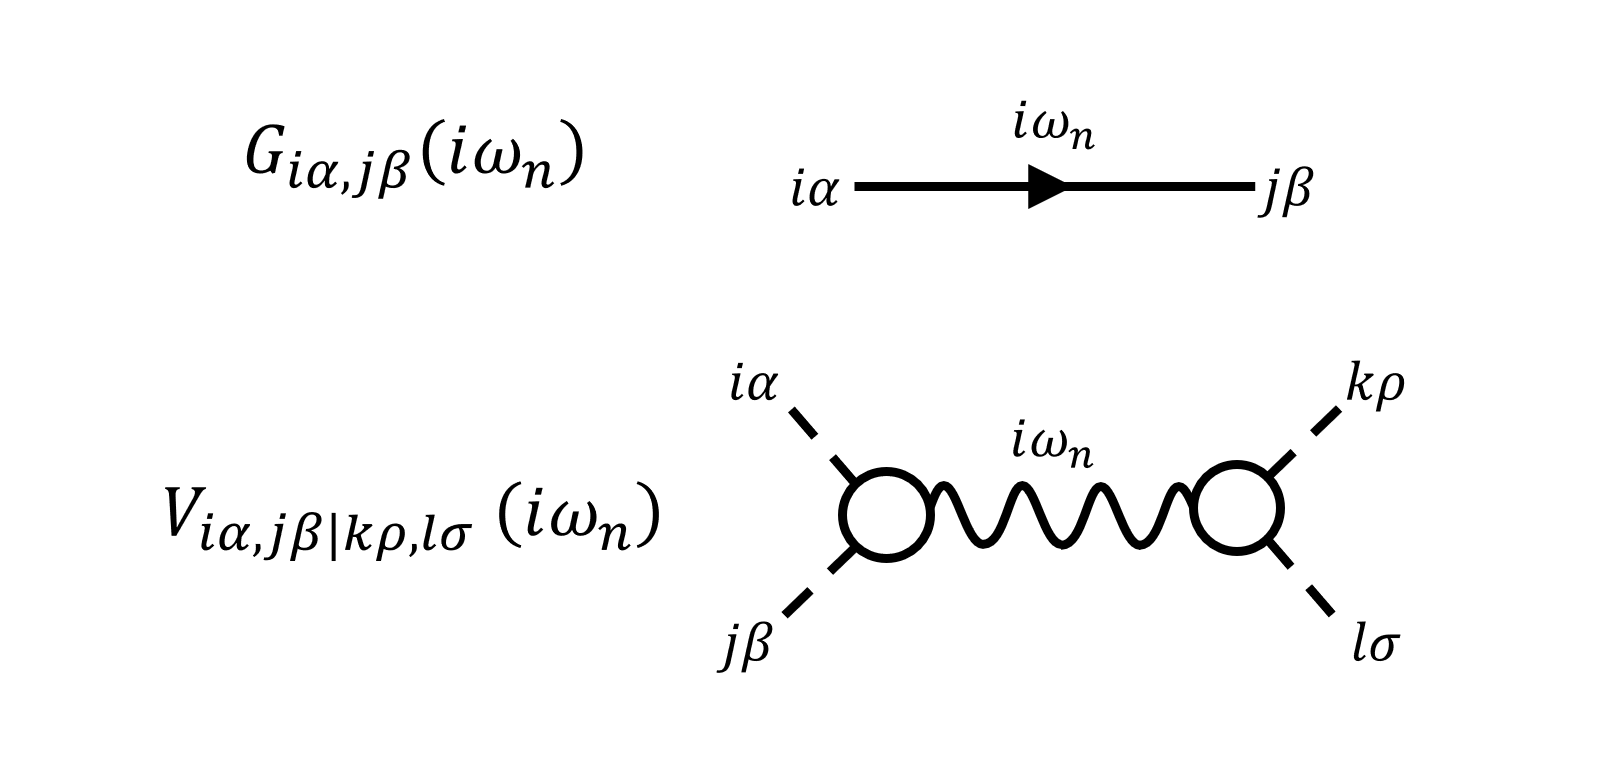
\includegraphics[width=0.8\textwidth]{Semion_diagram_elements.png}
	\caption{Графические изображения для семионной диаграммной техники.}	
\end{figure}

Задача исследования равновесной термодинамики гамильтониана \eqref{eq:Ham_semion} может быть  описана непосредственно через стандартную Мацубаровскую диаграммную технику \cite{AGD} со следующими правилами:
\begin{itemize}
	\item выражении для функции Грина невзаимодействующих семионов
	\begin{equation}
	\label{eq:Semion_Green_function}
	\begin{split}
		G_{i\alpha,j\beta}(i\omega_n) & := \left\langle T_\tau \left\{ c_{i\alpha} c^\dagger_{j\beta} \right\} \right\rangle 
		\equiv \delta_{ij} \left( i\omega_n - \xi_i \sigma^z_{\alpha\beta} + \mu_0 \right)^{-1} = \\ & = \delta_{ij} \frac{ i\omega_n +\mu_0 + \xi_i \sigma^z_{\alpha\beta} }{ \left( i\omega_n +\mu_0 \right)^2 - \xi_i^2 }
	\end{split}
	\end{equation}Традиционно, многочастичные функции Грина могут быть выражены через двухчастичную с помощью теоремы Вика.
	
	\item Выражение для вершины взаимодействия
	\begin{equation}
		\label{eq:Semion_interaction_vertex}
		V_{i\alpha, m\beta|j\rho, n\eta}(i\omega_n) = - \frac{2 g}{K} \cdot \delta_{im} \delta_{jn} J_{ij} \frac{1}{4} (\sigma^x_{\alpha \beta} \sigma^x_{\rho \eta} + \sigma^y_{\alpha \beta} \sigma^y_{\rho \eta}) \cdot \theta\left( \varepsilon_0 - |\omega_n| \right)
	\end{equation}
	где $J_{ik}$ -- матрица смежности $K$-регулярного графа, на котором определена задача. Зависимость от частоты диктуется Куперовской природой взаимодействия и отражает тот факт, что характерные передачи энергии не превышают $\varepsilon_0$, что и отражает наличие $\theta$-функции Хевисайда.
	
	\item В каждой точке встречи линий по всем индексам производится свёртка: суммирование латинских индексов по всем узлам и свёртка по спиновым греческим индексам.
	
	\item В точках соединения линия выполняется закон сохранения Мацубаровских частот: сумма всех исходящих равна сумме всех входящих. По незафиксированным законами сохранения и не относящимся ко внешним линиям диаграммы частотам происходит суммирование.
	
	\item Вычисление разновременных корреляторов различных операторов производится стандартным образом --- выражением этих корреляторов через многочастичные функции Грина и подсчётом соответствующей диаграммы.
\end{itemize}
Графические обозначения элементов техники представлены на Рис. \ref{fig:Semion_diagram_technique}.

\subsubsection{Учёт параметра порядка в семионной диаграммной технике}
У Мацубаровской техники в исходной редакции есть существенный недостаток: она плохо отражает  качественную перестройку основного состояния, происходящую при сверхпроводящем переходе. Однако, ситуацию можно исправить, воспользовавшись идеей в духе среднего поля. Именно, рассмотрим стандартную диаграммную технику Мацубары для гамильтониана \eqref{eq:Ham_semion_with_self_consistency}, но теорию возмущений будем строить по новому гамильтониану взаимодействия $H^F_{int}$. В таком случае, выражения \eqref{eq:Semion_Green_function} и \eqref{eq:Semion_interaction_vertex} изменятся, соответственно, следующим образом:
\begin{equation}
	\label{eq:Semion_Green_function_with_OP}
	\begin{split}
		G_{i\alpha,j\beta}(i\omega_n) & = \delta_{ij} \left( i\omega_n - \xi_i \sigma^z_{\alpha\beta} - \sum_k \widetilde{\Delta}^k_i \sigma^k_{\alpha\beta} + \mu_0 \right)^{-1} = \\ & = \delta_{ij} \frac{ i\omega_n +\mu_0 + \xi_i \sigma^z_{\alpha\beta} - \sum_k \widetilde{\Delta}^k_i \sigma^k_{\alpha\beta} }{ \left( i\omega_n +\mu_0 \right)^2 - \xi_i^2 - \left| \widetilde{\Delta}_i \right|^2 }
	\end{split}
\end{equation}
\begin{equation}
	\label{eq:Semion_interaction_vertex_with_OP}
		V_{i\alpha, m\beta|j\rho, n\eta}(i\omega_n) = - \frac{2 g}{K} \cdot \delta_{im} \delta_{jn} J_{ij} \cdot \sum_k \frac{1}{4} \left( \sigma^k_{\alpha \beta} - \mathcal{C}^k_i \delta_{\alpha\beta} \right) \left( \sigma^k_{\rho \eta} - \mathcal{C}^k_j \delta_{\rho\eta} \right)
\end{equation}
где $\widetilde{\Delta}$ --- параметр порядка, определяемый из уравнения самосогласования \eqref{eq:Order_paramter_self_consistency}, а $\mathcal{C}$ --- все то же термодинамическое среднее для задачи спина в постоянном магнитном поле, определяемом значением $\widetilde{\Delta}$. Постоянное слагаемое $E^F_0$ является температурно-зависимой сдвижкой энергии, так что его наличие влияет аддитивным образом лишь на свободную энергию и её температурные производные. Кроме перечисленных выше модификаций, правила техники не изменяются. 

Эта техника работает по параметру $1/K$, и является последовательным способом выяснять степень применимости седлового приближения.

\subsubsection{Диаграммная техника для поля параметра порядка}
Другим способом исследовать задачу является рассмотрение диаграммного ряда теории возмущений непосредственно для пропагатора флуктуаций параметра порядка. Изложение этой техники в формализме диаграммной техники Келдыша имеется в \cite{Kiselev_Oppermann_2000}.
\begin{enumerate}
	\item Определим флуктуацию следующим образом:
	\begin{equation}
	\label{eq:Order_paramter_fluctuation_definition}
	r^k_i(\tau) := \Delta^k_i(\tau) - \widetilde{\Delta}^k_i
	\end{equation}
	где $\widetilde{\Delta}$ --- параметр порядка, определяемый из уравнения \eqref{eq:Order_paramter_self_consistency}.
	
	\item Используя формулу
	$$
	\ln \det \left( L_0 + \delta L \right) = \ln \det L_0 + \ln \det \left( 1 + L_0^{-1} \delta L \right)
	$$
	бозонное действие \eqref{eq:Boson_action} можно переписать в виде:
	\begin{align*}
	\mathcal{A}_{b} \left[ \Delta \right] & = \mathcal{A}_{b} \left[ \widetilde{\Delta} \right] + \int\limits_{0}^{\beta} d\tau \left[ 2 \left(\frac{K}{2g}\right) \sum_{ij} \sum_k r^k_i J^{-1}_{ij} r^k_j \right] - \ln \det \left( 1 + G \delta L \right) \\
	\delta L & = - \sum_i \sum_k \sigma^k_{\alpha\beta} r^k_i \\
	\end{align*}
	где оператор $L_0^{-1}$ есть функция Грина семионной задачи с учётом параметра порядка \eqref{eq:Semion_Green_function_with_OP}.
	
	\item Далее, используя тождество
	$$
	\ln \det (1 + A) = \Tr \ln (1 + A) \equiv \sum_{n = 1}^\infty \frac{(-1)^{n-1}}{n} \Tr \left[A^n\right]
	$$
	перепишем $r$-зависимую часть действия в форме
	\begin{equation*}
	\mathcal{A}_b[r] = \int\limits_{0}^{\beta} d\tau \left[ 2 \left(\frac{K}{2g}\right) \sum_{ij} \sum_k r^k_i J^{-1}_{ij} r^k_j \right] - \sum_{n = 1}^\infty \frac{1}{2n} \Tr \left[- \left(L_0^{-1} \delta L \right)^n\right]
	\end{equation*}
	где учтено, что все нечётные порядки старше первого в сумме обнулятся после взятия функционального интеграла в силу нечётности по полям $r$. Обращение в нуль первого порядка этого ряда эквивалентно выполнению уравнения самосогласования \eqref{eq:Order_paramter_self_consistency} по определению.
	
	\item Наконец, заметим, что выражение под знаком суммы имеет очевидную интерпретацию в терминах Мацубаровской диаграммной техники с учётом параметра порядка, описанной выше: диаграмма, соответствующая выражению $F_n[r] := \Tr \left[- \left(L_0^{-1} \delta L \right)^{2 n}\right]$,  показана на Рис. \ref{fig:n_particle_renormed_vertex}. Она представляет из себя отклик $n$-го порядка на переменное внешнее поле. 
	\begin{figure}[h]
		\label{fig:n_particle_renormed_vertex}
		\centering
		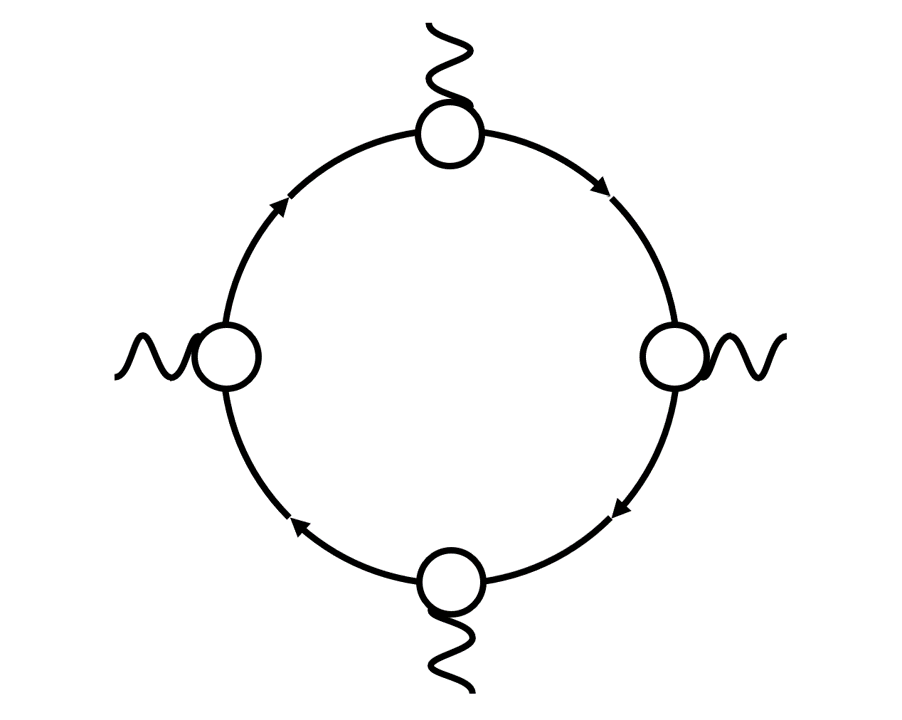
\includegraphics[width=0.5\textwidth]{N_particle_renormed_vertex.png}
		\caption{Диаграммное представление для слагаемого $n$-го порядка в действии, обозначенного в тексте как $F_n[r]$. На рисунке $n = 2$.}
	\end{figure}
	Определим также ядро этого отклика $R[n]_{ij}^{mn}\left(\tau_1,...\tau_{2n}\right)$, даваемое диаграммой на Рис. \ref{fig:n_particle_renormed_vertex}, но с усечёнными бозонными концами (т. е. просто фермионной петлёй с $2n$ вершинами в виде операторов спина). Очевидно, $R[n]$ зависит лишь от разностей времён, т. е. от $2n-1$ переменных.
	%TODO: PROP make a better description of R[n] diagram
	
	\item Таким образом, пока что полученная диаграммная техника представляет из себя задачу изучения бозонного поля с многочастичным взаимодействием. При этом следует явно отщепить слагаемое с $n = 1$, которое даёт вклад непосредственно в пропагатор поля флуктуаций $r$. Поскольку квадратичная часть действия в функциональном интеграле однозначно определяется обратной функции Грина невозмущенной задачи, то имеем тогда для пропагатора:
	\begin{equation}
	\label{eq:Order_parameter_fluctuations_propagator_definition}
		\begin{split}
			D^{mn}_{ij}(\tau) & := \left\langle T_\tau \left\{ \delta^k_i(\tau_0)    	\delta^k_i(\tau_0 + \tau) \right\} \right\rangle = \\
			& = \left[ 2 \times \frac{K}{2g} J_{ij}^{-1} \delta^{mn} - 2 \times \frac{1}{2} R[1]_{ij}^{mn}(\tau) \right]^{-1}
		\end{split}
	\end{equation}
	
	\item Итоговая диаграммная техника формулируется в терминах элементов $D$ и $R[n]$: $k$-ый порядок теории возмущении соответствует сумме всевозможных диаграмм, составленных из семионных петлей с различным чётным числом вершин $2k$ и флуктуационных пропагаторов \eqref{eq:Order_parameter_fluctuations_propagator_definition}, соответствующих волнистой линии в исходной Мацубаровской диаграммной технике для семионов. Каждая семионная петля порядка $2k$ при этом имеет дополнительный коэффициент $1/{2k}$.
\end{enumerate}  

Отметим, в частности, что обрезание теории возмущений на 4-ом порядке, что означает учёт единственной диаграммы с вершиной $\frac{1}{4}R[2]$, соответствует формализму теории Гинзбурга Ландау. Таким образом, величина петель $R[n]$ на нулевой переданной частоте задаёт коэффициенты функционала Гинзбурга-Ландау. При этом, как и раньше, тензорная инвариантность, которой по построению обладают все диаграммы, напрямую связана с калибровочной $U(1)$-инвариантностью задачи сверхпроводимости.


\subsection{Некоторые заключительные физические замечания}
Важным физическим примечанием будет соответствие полученных результатов общепринятой картине описания сверхпроводимости как нарушения зарядовой $U(1)$-симметрии: компоненты введённого бозонного векторного поля соответствуют действительной и мнимой части комплексного параметра порядка, рассматриваемого в теории сверхпроводимости. В частности, такая картина хорошо соотносится с очевидной вращательной инвариантностью полученного уравнения самосогласования \eqref{eq:Order_paramter_self_consistency}. Например, в данную теорию легко ввести внешнее электромагнитное поле методом минимального спаривания. Краткое обсуждение соответствия симметрийных аспектов теории имеется в работе \cite{Poboiko_Feigelman_Paraconductivity}.

Следующим важным физическим комментарием будет вопрос о критерии применимости метода стационарной фазы, формализма среднего поля и прочих родственных вещей. Строго говоря, все эти методы работают по параметру $1/K$, и в общем случае необходимо следить за взаимодействиями эффектов одного порядка при попытках выяснять поправки к среднеполевым ответам. Качественно, отклонения от среднеполевой картины появляются за счёт двух эффектов:
\begin{itemize}
	\item Флуктуаций параметра порядка вокруг своих средних, определяемые конечным числом соседей. Эти явления мы опишем далее.
	
	\item Эффекты неоднородностей, вносимые распределением энергий $\xi_i$ на узле, которые также уменьшаются с увеличением числа соседей. Влияние этих неоднородностей сказывается на этапе решения уравнения самосогласования, и потому их учёт является отдельной сложной задачей.
\end{itemize}
Предел $K \rightarrow \infty$, как показано в уравнении \eqref{eq:Order_parameter_self_consitency_BCS_limit}, соответствует стандартной модели БКШ, в рамках которой в системе развивается однородный параметр порядка, а все термодинамические характеристики системы, согласно теореме Андерсона, испытывают влияние беспорядка исключительно за счёт изменения одночастичной плотности состояний.

Наконец, заметим, что полученные результаты могут быть также воспроизведены с помощью формализма аномальных средних Намбу-Горькова, изложенного, например, в \cite{AGD}. Между этим и приведённым в данной работе формализмом имеется простое соответствие: средние операторов $s^{x,y}$ на узле соответствуют Горьковских аномальным средним вида $\left\langle a^\dagger a^\dagger \right\rangle$ в исходной задаче взаимодействующих электронов, в то время как оператор $s^z$ несёт информацию о диагональной части функции Грина и, соответственно, средних вида $\left\langle a^\dagger a\right\rangle$. 



%\section{Исследование решения уравнения самосогласования}
%TODO: DERIVE subsubsection{1/K-диграммная техника для параметра порядка} -- если она вообще существует



\section{Изучение свойств низкоэнергетических мод}
Нашей задачей будет изучение низкоэнергетических возбуждений над основным состоянием системы при низкой температуре $T << T_c$. При этом мы считаем, что этих возбуждений при низких температурах очень мало, а потому их взаимодействием можно пренебречь, что соответствует рассмотрению в функциональном интеграле только квадратичной по флуктуациями части бозонного действия. В таком случае, возбуждения  описываются своим пропагатором \eqref{eq:Order_parameter_fluctuations_propagator_definition}, который очевидным образом содержит все одночастичные свойства этих возбуждений.

\subsection{Связь свойств флуктуаций с их функцией Грина}
\subsubsection{Локальная плотность состояний}
В первую очередь, нас интересует статистика локальной плотности состояний на узле $\rho_i(\omega)$ этих возбуждений при низких частотах. Определение этой величины и ее связь с функцией Грина следующие:
\begin{equation}
	\label{eq:LDoS_through_GF}
	\rho_i(\omega)  := \lim_{M \rightarrow \infty} \sum_i \sum_\alpha \left| \psi^\alpha_i \right|^2 \delta(\omega - \varepsilon^\alpha) =  \lim_{\gamma \rightarrow +0} \lim_{M \rightarrow \infty} \frac{1}{\pi} \Im D_{ii}(\omega + i \gamma)
\end{equation}
где $\varepsilon^\alpha$ -- энергия возбуждения с волновой функцией $\psi^\alpha$, а также введено инфинитезимальное уширение уровней $\gamma$, отвечающее за корректный переход к термодинамическому пределу $M \rightarrow \infty$ или, эквивалентно, за регуляризацию входящей в определение локальной плотности состояний $\delta$-функции от энергии.

Как следует из определения, $\rho_i$ показывает вероятность наличия на данном узле состояния с заданной энергией $\omega$. В частности, именно эта величина будет определять исход эксперимента по туннельной микроскопии (а точнее, её среднее на масштабе порядка размера иглы). Очевидно, что в металлической системе эта величина совпадает со стандартной плотностью состояний, которая в нашей модели задаётся беспорядком и равна $1/2$. 

Важно, однако, отметить, что с интерпретацией этой величины как буквально локальной \textit{в реальном пространстве} плотности состояний следует быть осторожным, поскольку определённая в \eqref{eq:LDoS_through_GF} величина является плотностью состояний \textit{на одном узле графа}, который, в свою очередь, соответствует одноэлектронному локализованному состоянию, занимающему некоторый конечный корреляционный объём. При этом взаимное пространственное расположение различных состояний, соответствующее различным узлам графа, является отдельной задачей, поэтому физический смысл эта величина имеет лишь как среднее по масштабу меньше или порядка локализационного объёма $V_{loc}$.

\subsubsection{Inverse Participation Ratio}
Ещё одной характеристикой возбуждений, статистика которой нас будет интересовать, является т. н. Inverse Participation Ratio (далее IPR), характеризующая объём, который занимает соответствующая волновая функция. Её формальное определение и связь со свойствами функции Грина выглядят следующим образом:
\begin{equation}
	\label{eq:IPR_through_GF}
	L(\omega) := \lim_{M \rightarrow \infty} \sum_i \sum_\alpha \left| \psi^\alpha_i \right|^4 \delta(\omega - \varepsilon^\alpha) = \lim_{\gamma \rightarrow +0} \lim_{M \rightarrow \infty} \frac{\gamma}{\pi} \left| D_{ii}(\omega + i \gamma) \right|^2 
\end{equation}
Как буквально следует из определения, эта величина содержит в себе информацию о втором моменте амплитуды волновой функции, усреднённом по всем узлам системы $i$ и всем состояниям $\alpha$  с заданной энергией $\omega$.

Основным свойством IPR является то, что в термодинамическом пределе $m \rightarrow 0$ она равна 0, если состояния делокализованы, и некоторому конечному числу $\sim V_{loc}^{-1} $, если у состояний имеется конечный локализационный объём $V_{loc}$. 

Здесь также следует отметить, что нужно с осторожностью интерпретировать эту величину как характеристику структуры возбуждений в реальном пространстве из-за сложного взаимного расположения одночастичных электронных состояний, соответствующих различным узлам графа. Однако, у этой величины, тем не менее, имеется конкретный физический смысл: поскольку локализация в пространстве узлов по построению модели означает локализацию в реальном пространстве в конечном объёме $\sim V_{loc}$, то возбуждения с таким свойством не будут непосредственно приводить к диссипации энергии.


\subsection{Выражение для пропагатора флуктуаций параметра порядка}
Для начала установим явный вид пропагатора флуктуаций. Схожие вычисления в формализме диаграммной техники Келдыша можно найти в работе \cite{Poboiko_Feigelman_Paraconductivity}. 
Явный вид фермионной петли $R[1]$:
\begin{equation*}
	\begin{split}
		R[1]_{ij}^{mk}(i\omega_n) & = -T \sum_{\epsilon_n} \left[ G_{i\alpha,j\beta}(i\omega_n + i \epsilon_n) \frac{1}{2}\sigma^m_{\beta\rho} G_{j\rho,i\eta}(i \epsilon_n) \frac{1}{2} \sigma^m_{\eta\alpha} \right] = \\
		& = -\frac{1}{2} \delta_{ij} \frac{\tanh(\beta h)}{2 h} \left[ -\frac{ h^2 \delta^{mk} }{ h^2 + \frac{\omega_n^2}{4} } + \frac{ \omega_n h^s \epsilon^{smk} + 2 h^m h^k - h^2 \delta^{mk} }{h^2 + \frac{\omega_n^2}{4}} \right]
	\end{split}
\end{equation*}
где
$$
h^x_i = \widetilde{\Delta}^x_i, h^y_i = \widetilde{\Delta}^y_i, h^z_i = - \xi_i, h^2 = \left| \widetilde{\Delta}_i \right|^2 + \xi_i^2
$$
Обращаем внимание, что частотный аргумент петли и пропагатора $\omega_n$ представляет из себя бозонной Мацубаровскую частоту, а внутренняя частота петли $\varepsilon_n$ --- фермионную. Используя формулу \eqref{eq:Order_paramter_fluctuation_definition}, выпишем явный вид обратного пропагатора:
\begin{equation}
	\label{eq:Order_parameter_fluctuation_inverse_propagator_explicit}
	\begin{split}
		\left[ D^{mk}_{ij}(i \omega_n) \right]^{-1} & =  2\left[ \frac{K}{2g} J_{ij}^{-1} \delta^{mk} - \frac{1}{2} R[1]_{ij}^{mk}(i\omega_n) \right] = \\
		& = \frac{K}{g} J_{ij}^{-1} \delta^{mk} + \delta_{ij} \frac{\tanh(\beta h)}{h} \left[ \frac{ h^m h^k - h^2 \delta^{mk} }{h^2 + \frac{\omega_n^2}{4}} + \frac{ \frac{\omega_n}{2} h^s \epsilon^{smk} }{h^2 + \frac{\omega_n^2}{4}} \right]
	\end{split}
\end{equation}
Симметричная по $m,k$ часть этого выражения содержит в себе информацию о функции Грина двух мод флуктуаций: поперечной и продольной, соответственно тому, как направления колебаний соотносятся с направлением параметра порядка. В терминах комплексного параметра порядка это соответствует фазовой моде Голдстоуна и амплитудной моде Хиггса. Недиагональный же член несёт в себе информацию о смешивании двух мод между собой.

Заметим, что \textit{всегда} имеется хотя бы одно поперечное возбуждение с $\omega = 0$, поскольку оно является следом нарушенной $U(1)$-симметрии: уравнение самосогласования \eqref{eq:Order_paramter_self_consistency} инвариантно относительно этой симметрии, и в частности, относительно инфинитезимально малых поворотов параметра порядка на некоторый угол без изменения модуля, что и соответствует описанному возбуждению.


\subsection{Итоговая задача изучения низкоэнергетических поперечных мод}
Чтобы сделать задачу более конкретной, примем ряд дальнейших упрощений:
\begin{enumerate}
	\item Поскольку нас интересуют низкоэнергетические моды, то далее будем считать $\omega_n \ll |\Delta|$. Как следствие, взаимодействием продольной и поперечной мод можем пренебречь
	\item В рамках теории сверхпроводимости для чистого металла, Хиггсовская мода должна быть массивной, что соответствует наличию щели в низкоэнергетическом спектре продольных возбуждений. Некоторые расчёты, качественно обосновывающие данное приближение, имеются в работе \cite{Shtyk_Feigelman_2017}. Поэтому мы будем считать, что такая картина сохраняется и далее, так что в дальнейшем будем изучать только поперечную моду. 
	\item Также сделаем одно упрощение, касающееся статистики поля параметра порядка $\widetilde{\Delta}$. Для дальнейших расчётов мы будем считать, что его значение на каждом узле \textit{равно своему значению в пределе теории БКШ \eqref{eq:Order_parameter_BCS_limit}}. Мотивация этого приближения состоит в следующем: 
	\begin{enumerate}
		\item[а.] ранее для этой задачи уже были проведены оценки типичных значений $K$, при которых будет происходить основная физика \cite{FI_microwave}. Мы ещё вернёмся к этим оценкам.
		\item[б.] Эти оценки, по данным \cite{Feigelman_et_al_2010}, лежат в области, где параметр порядка флуктуирует довольно слабо. 
	\end{enumerate}
	Таким образом, роль беспорядка в этом приближении сводится только к непосредственному влиянию величин $\xi_i$, явным образом входящего в выражение петли $R[1]$, определяющей флуктуационный пропагатор \eqref{eq:Order_parameter_fluctuation_inverse_propagator_explicit}. Сделаем пару важных замечаний:
	\begin{enumerate}
		\item[а.] строго говоря, это приближение не вполне обоснованно, так как лидирующий порядок изучаемых эффектов есть $1/K$, равно как и порядок флуктуаций параметра порядка. Однако мы надеемся, что качественная картина от этого не изменится. В дальнейшем это приближение будет явно проверено.
		\item[б.] Важным замечанием является также и то, что игнорирование истинного распределения параметра порядка приводит к потере симметрийной поперечной моды с $\omega = 0$, описанной ранее.
	\end{enumerate}
\end{enumerate}

Теперь можно дать окончательную формулировку задачи, которую мы собираемся далее решать, и которая должна описывать появление в сверхпроводнике низкоэнергетических возбуждений. А именно, мы хотим выяснить статистику локальной плотности состояний \eqref{eq:LDoS_through_GF} и IPR \eqref{eq:IPR_through_GF} собственных мод \textit{на нулевой энергии} для линейного оператора 
\begin{equation}
	\label{eq:Investigated_linear_operator}
	A_{ij}(\omega) = \frac{K}{g} J_{ij}^{-1} - \delta_{ij} \eta_i (\omega)
\end{equation}
где величина $\eta_i$ определяется формулой
\begin{equation}
	\label{eq:eta_definition}
	\eta_i(\omega) = \frac{ \sqrt{ |\Delta_i|^2 + \xi_i^2 } }{ |\Delta_i|^2 + \xi_i^2 - \frac{\omega^2}{4} }
\end{equation}
а величины $\Delta_i$ все являются одинаковыми и задаются как параметр модели формулой \eqref{eq:Order_parameter_BCS_limit}. Поясним, что нас интересует именно нулевое собственное значение, так как, согласно формулам \eqref{eq:LDoS_through_GF}-\eqref{eq:IPR_through_GF}, вся информация содержится буквально в операторе $A^{-1}$, что соответствует его функции Грина $G(E) = (E - A)^{-1}$ именно при $E = 0$. Реальная физическая энергия возбуждений входит в задачу как параметр $\omega$.


\subsection{Основные изучаемые характеристики ансамбля}
Напомним, что в конечном итоге мы интересуемся статистическими свойствами ансамбля, задаваемого присутствующими в определении \eqref{eq:Investigated_linear_operator} случайностями. Для этого удобно ввести две величины, в значительной степени характеризующие распределение -- среднее и типичное значение:
$$ x_{mean} := \langle x \rangle $$
$$ x_{typ} := \exp \langle \ln x \rangle $$
где $\langle \cdot \rangle$ означает усреднение по ансамблю. Эти величины обладают следующими качественными свойствами:
\begin{itemize}
	\item среднее значение, как известно благодаря центральной предельной теореме, характеризует то, как устроены самоусредняющиеся в реальном образце аддитивные величины.
	\item В тоже время типичное значение характеризует те вещи, которые являются существенно локальными, и потому чувствительны к конкретной реализации. Математически это выражается в том, что, поскольку логарифм -- медленная функция, то типичное значение, согласно своему названию, будет близко к положению максимума функции распределения, т. е. к значению, которое будет реализовываться чаще всего.
\end{itemize}


\subsection{Связь поставленной задачи с локальными свойствами}
К сожалению, поставленная задача об исследовании функции Грина оператора \eqref{eq:Investigated_linear_operator} обладает тем недостатком, что она нелокальна по узлам: в общем случае матрица $J^{-1}$ имеет большое число ненулевых матричных элементов, так что каждый узел исходного графа связан с большим число других узлов, в том числе находящихся от него на большом расстоянии по графу. Однако, если интересоваться лишь фактом \textit{наличия} конечной в термодинамическом пределе плотности возбуждений, то оказывается, что задачу можно свести к локальной. Делается это следующим образом:
\begin{enumerate}
	\item Обозначим
	$$
	\hat{\eta}_{ij} = \delta_{ij} \eta_i, \hat{R}_{ij} = \frac{g}{K} J_{ij}
	$$
	Также введём оператор
	\begin{equation}
		\label{eq:Local_operator_definition}
		\hat{C} = \sqrt{\hat{\eta}} \hat{R} \sqrt{\hat{\eta}}
	\end{equation}
	и его функцию Грина на собственном значении $1$ с некоторым уширением уровней:
	\begin{equation}
		\label{eq:Local_operator_Green_function_definition}
		\hat{G}(\gamma) = \left( \left[ 1 + i \gamma \right] - \hat{C} \right)^{-1} 
	\end{equation}
	Под числами здесь подразумеваются соответствующие скалярные матрицы, пропорциональные единичной.
	Далее будет продемонстрировано, что интересующая нас задача может быть сведена к исследованию \textit{локального} оператора $\hat{C}$ и его функции Грина $\hat{G}$
	\item Проделаем следующие преобразования над флуктуационным пропагатором $D$:
	\begin{equation}
		\label{eq:Connection_between_GF}
		\begin{split}
			D(\gamma \rightarrow +0) & \equiv \left( \hat{A} + i 0 \right)^{-1} \overset{\eqref{eq:Investigated_linear_operator}}{=} \left( \hat{R}^{-1} - \hat{\eta} + i 0 \right)^{-1} \equiv \\
			& \equiv \sqrt{\hat{\eta}} \hat{R}  \left( \sqrt{\hat{\eta}} \hat{R} \sqrt{\hat{\eta}} - \sqrt{\hat{\eta}} \hat{R} \left[ \hat{\eta} - i 0 \right] \hat{R} \sqrt{\hat{\eta}} \right)^{-1} \hat{R} \sqrt{\hat{\eta}} = \\
			& = \hat{C} \hat{\eta}^{-1/2} \left( \hat{C} - \hat{C}\left[1 - i 0 \hat{\eta}^{-1} \right] \hat{C} \right)^{-1} \hat{\eta}^{-1/2} \hat{C} = \\
			& = \hat{C} \hat{\eta}^{-1/2} \underset{\hat{G}(+0)}{\underbrace{  \left( \left[1 - i 0 \hat{\eta}^{-1} \right]^{-1} - \hat{C} \right)^{-1}  }} \left[1 - i 0 \hat{\eta}^{-1} \right]^{-1} \hat{C}^{-1} \hat{\eta}^{-1/2} \hat{C} = \\
			& = \left/ \hat{\eta}^{-1} > 0 \right/ = \hat{C} \hat{\eta}^{-1/2} \hat{C}^{-1} \hat{C} \hat{G}(+0) \hat{C}^{-1} \hat{\eta}^{-1/2} \hat{C} = \\
			& = \left/ \hat{C} = 1 + i0 - \hat{G}(+0)^{-1} \right/ = \\
			& = \hat{C} \hat{\eta}^{-1/2} \hat{C}^{-1} \left( \hat{G}(+0) - 1 \right) \hat{C}^{-1} \hat{\eta}^{-1/2} \hat{C}
		\end{split}
	\end{equation}
	При преобразованиях использовалось условие $\hat{\eta} > 0$, означающее положительную определённость соответствующей матрицы. Также операторы $\hat{R}, \hat{\eta}$ считались обратимыми: матрица $\hat{\eta}$ и все её ненулевые степени обратимы из-за положительной определённости, а обратимость матрицы $\hat{R} \propto J$ уже обсуждалась ранее.
	
	\item В таком случае, для локальной плотности состояний возбуждений верно следующее:
	\begin{equation}
		\label{eq:Connection_of_LDoS_with_Im_part_of_local_GF}
		\begin{split}
			\rho_i & \equiv \frac{1}{\pi} \Im \left\langle i \right| D \left| i \right\rangle = \frac{1}{\pi}\Im \left\langle i \right| \hat{C} \hat{\eta}^{-1/2} \hat{C}^{-1}  \left( \hat{G}(+0) - 1 \right) \hat{C}^{-1} \hat{\eta}^{-1/2} \hat{C} \left| i \right\rangle = \\
			& = \left/ \hat{C}_{ij}, \hat{\eta}_{ij} \in \mathbb{R} \right/ = \left\langle i \right| \hat{C} \hat{\eta}^{-1/2} \hat{C}^{-1} \left[ \frac{1}{\pi}\Im \hat{G}(+0) \right] \hat{C}^{-1} \hat{\eta}^{-1/2} \hat{C} \left| i \right\rangle = \\
			& =  \left/ C^{-1} \left[ \Im \left(\lambda + i0 - C \right)^{-1} \right] C^{-1} = \frac{1}{\lambda^2} \left[ \Im \left(\lambda + i0 - C \right)^{-1} \right] \right/ = \\
			& = \left\langle i \right| \hat{C} \hat{\eta}^{-1/2} \left[ \frac{1}{\pi}\Im \hat{G}(+0) \right] \hat{\eta}^{-1/2} \hat{C} \left| i \right\rangle \equiv \\
			& \equiv \frac{1}{\eta_i} \left\langle i \right| R \left[ \frac{1}{\pi}\Im \hat{G}(+0) \right] R \left| i \right\rangle
		\end{split}
	\end{equation}
	Поскольку операторы $R$ предполагаются обратимыми, то из этой формулы можно сделать следующий вывод: \textit{у исходного оператора \eqref{eq:Investigated_linear_operator} существует локальная плотность состояний тогда и только тогда, когда существует ненулевая плотность собственных состояний оператора $C$ с собственным числом 1}.
	
	\item Наконец, рассмотрим связь между IPR для двух задач. Поскольку нас интересует IPR в случае с конечной плотностью состояний, то чтобы предел $\gamma \rightarrow 0$ в определении IPR \eqref{eq:IPR_through_GF} был отличен он нуля, необходимо, чтобы малость $\gamma$ компенсировала вещественная часть функции Грина:
	\begin{equation}
		\label{eq:Condition_on_GF_real_part_for_localized_states}
		L > 0 \Rightarrow \lim_{\gamma \rightarrow 0} \lim_{M \rightarrow \infty} \left| \Re D_{ii} \right| = \infty
	\end{equation}
	В таком случае, верно следующее: \textit{свойство локализации собственных мод интересующего нас оператора \eqref{eq:Investigated_linear_operator} имеется тогда и только тогда, когда это свойство наличествует у собственных мод локального оператора \eqref{eq:Local_operator_definition} с единичным собственным числом}.
\end{enumerate}
Итогом этих рассуждения является следующее важное следствие: качественные характеристики, такие как наличие конечной плотности состояний и локализация низкоэнергетических возбуждений, задаваемых оператором \eqref{eq:Investigated_linear_operator}, можно изучать по аналогичным свойствам локального оператора \eqref{eq:Local_operator_definition}. А потому исследование может быть переведено в плоскость исследования функции Грина локального оператора \eqref{eq:Local_operator_Green_function_definition} на единичном собственном числе. 
Подчеркнём, однако, что полученное сопоставление не сохраняет численные значения, а потому, строго говоря, может потенциально вносить некоторые дополнительные параметрические зависимости в получаемые ответы.


\subsection{Качественные предсказания о поведении локальной модели}
Прежде чем приступить к исследованию новой локальной задачи, необходимо упомянуть, что задача изучения локального оператора \eqref{eq:Local_operator_definition} в интересующей нас связи была сформулирована в работе \cite{FI_microwave}, и там же был сделан ряд качественных и количественных предсказаний касательно поведения этой модели, которые мы сейчас кратко изложим. Основный их смысл состоит в наличии \textit{двух характерных значений параметра $K$} со следующими свойствами:
\begin{enumerate}
	\item Точка
	\begin{equation}
		\label{eq:K2_definition}
		K_2 = \frac{g}{4} \exp \left\{ \frac{1}{g} \right\}
	\end{equation}	
	характеризует значение $K$, начиная с которого (при движении из бесконечных $K$) в системе появляются низкоэнергетические моды со сколь угодно низкой энергией.
	\item Точка
	\begin{equation}
		\label{eq:K1_definition}
		K_1 = g \exp \left\{ \frac{1}{2g} \right\}
	\end{equation}
	характеризующая момент, начиная с которого (при движении из бесконечных $K$) возбуждения со сколь угодно низкой энергией становятся делокализованными.
	\item В работе также исследована асимптотика положения этих точек на малых частотах $\omega \ll \Delta$. Утверждается, что она может быть описана как
	$$
	K_1(\omega) = K_1(0) \left(1 + \frac{1}{\sqrt{6}g} \frac{\omega}{2 \Delta} \right)
	$$
	$$
	K_2(\omega) = K_2(0) \left(1 + \frac{1}{2} \frac{\omega^2}{4 \Delta^2} \right)
	$$
\end{enumerate}
Заметим также, что с учётом результатов по исследованию поведения уравнения самосогласования \eqref{eq:Order_paramter_self_consistency} вблизи $T_c$, проведённого в работе \cite{Feigelman_et_al_2010}, предсказывается следующая картина при уменьшении $K$:
\begin{itemize}
	\item при достижении $K = K_2 \gg 1$ (самый большой масштаб для $K$ в задаче) появляются низкоэнергетические возбуждения. Но на момент появления они ещё локализованы, и поэтому не приводят к диссипации.
	\item При достижении $1 \ll K = K_1 \ll K_2$ низкоэнергетические моды делокализуются. Одновременно с этим, беспорядок вносит сильную неоднородность в поле параметра порядка, делая одноузельное распределение величины $\Delta$ по узлам крайне широким, так что в этой области приближение $\Delta = \const$ перестаёт быть применимым.
	\item Наконец, при достижении некоторого критического значения $1 \ll K = K_c \ll K_1$ беспорядок вносит критическую неоднородность в распределение параметра порядка, что разрушает сверхпроводящее состояние.
\end{itemize}
Таким образом, интересующая нас область $K \ge K_1$, которую должна описывать исследуемая нами модель, согласно этим предсказаниям, правильно описывает наблюдаемую экспериментально качественную картину. Дальнейшее исследование, проделанное в данной работе, в первую очередь проверяет сделанные выше утверждения.